\section{\textit{De Iure Naturae et Gentium} (1672-1684)}

    Samuel von Pufendorf (1632–1694) composed his influential treatise De Iure Naturae et Gentium with the conviction that the foundations of social life and moral duties arise from human nature itself. In this monumental work, he explicitly challenges Thomas Hobbes’s idea that the natural state of human beings is nothing but incessant conflict. Instead, Pufendorf insists there is a principle of sociability that predates the establishment of any civil government.

    \begin{itemize}
        \item \textbf{Against Hobbes}: Pufendorf rejects the notion that the state of nature is a state of war. He instead highlights that human beings, by their very constitution, have social inclinations that foster mutual assistance and collaboration.
        \item \textbf{Principle of Society}: This intrinsic sociability or principle of society exists prior to, and independently of, any instituted government. For Pufendorf, it is not merely contractual arrangements that keep us together, but a profound sense of our own weakness and a recognition of the benefits of cooperating with others.
    \end{itemize}

    \subsection[On the Law of Nature in General]{Book II, Chapter III\\ 
                \textit{“On the Law of Nature in General”}}

        Within this segment, Pufendorf addresses how one should discern what constitutes the natural law—an enduring question for moral and political philosophers. His response hinges upon a careful observation of human nature, our fundamental needs, and our capacity for interaction.

        \subsubsection{Human being’s nature, condition and inclinations}

            \begin{quote}
                It seems to us that there is no more direct and appropriate way of discovering the natural law (\textit{jus naturale}) than to contemplate carefully human being’s nature, condition, and inclinations (\textit{quam ipsam hominis naturam, conditionem et inclinations accuratius contemplari}).
            \end{quote}

            Pufendorf contends that to grasp natural law—those norms valid universally, independent of any single political structure—we begin by looking inward. Human nature reveals both our desire to preserve ourselves and our innate vulnerability. Through these features, we see how a system of rules conducive to survival and cooperation arises.

        \subsubsection{Self-love}

            \begin{quote}
                The first thing that man has in common with all living things which are aware of themselves is that he loves himself to the highest degree (\textit{seipsum quam maxime amet}), is eager to preserve himself in every way, and strives to acquire those things that seem good to him and to repel those that seem evil. And this self-love, regularly speaking, is so very strong, as to supersede any inclination which man may have for another.
            \end{quote}

            He places self-love (amor sui) at the very core of humanity. We strive to avoid harm, acquire benefits, and secure our own well-being. Although this impulse is powerful, it does not inherently condemn us to hostility toward others. Rather, it prompts each individual to look after their own interests, which often demands external support from one’s peers. The strength of self-love explains why people sometimes appear egoistic, yet it also drives us to form relationships from which we derive advantage and assistance.

        \subsubsection{\textit{Summa imbecillitas}}
        
            \begin{quote}
                Besides this love of and eagerness to preserve himself by all means, we also find in man an extreme weakness (\textit{summa imbecillitas}) and a natural neediness (\textit{naturalis indigentia}). Hence, if we were to conceive him as abandoned to himself in this world without any assistance from other men, his life could seem to have been given him as a punishment.
            \end{quote}

            Pufendorf emphasizes the precarious condition of human life. We are physically vulnerable and generally incapable of thriving in isolation, especially when compared to many other creatures that rely on speed, strength, or other inherent defenses. In Pufendorf’s view, if left wholly alone—stripped of companionship and shared resources—our prospects for a comfortable life would be desperately poor. This recognition underlines our need for social bonds and cooperative networks.

        \subsubsection{Cooperation}

            \begin{quote}
                It is evident as well that, after the Divinity, no greater help and relief can come to a man than from other men. For even though we find the strength of individuals to preserve themselves so slight that they need the help of many things and men in order to live well and comfortably (since individuals would lack both the strength and the time to produce most of the things that are most useful and supremely necessary for men, if many men had not joined their efforts together), they can, on the other hand, still provide many things for the uses of others which they themselves do not need, and which would therefore be of no use to themselves if they were not dispensed to other men.
            \end{quote}

            From the preceding point about our extreme weakness flows the necessity of cooperating with others. Individual human beings can produce only so much on their own, both in terms of goods and labor. By working together, pooling resources, and exchanging services, we offset our inherent limitations. The knowledge that surplus resources held by one person might remedy the needs of another underscores how rational it is to seek forms of collaboration.

        \subsubsection{The foundation of the natural law}

            \begin{quote}
                Once these things have been established, it is easy to discover the foundation of the natural law. Man, it is clearly apparent, is an animal most eager to preserve himself, essentially in need, ill-equipped to maintain himself without the aid of those who are like him, and very well suited for the mutual promotion of advantages. All the same, he is often malicious, insolent (petulans), easily annoyed, and both ready and able to inflict harm.
            \end{quote}

            In these lines, Pufendorf deftly merges the contradictions of human nature. We are:

            \begin{itemize}
                \item Self-preserving but also fragile.
                \item Capable of altruism though we can be petulant or harmful when provoked.
            \end{itemize}

            The tension between mutual benefit and potential malice grounds the necessity of a moral and legal framework. Natural law emerges to regulate these interactions, ensuring that the drive for self-preservation is tempered by rules that enable stable cohabitation.

        \subsubsection{Sociability}

            \begin{quote}
                For this kind of animal to be safe and enjoy the goods that befall his worldly condition, it is necessary that he be sociable (necessarium est, ut sit sociabile). That is, he must will to be united with those who are similar to himself and conduct himself toward them in such a way that they are provided with no cause to hurt him, but instead have reason to maintain or promote his advantage.
            \end{quote}

            Pufendorf concludes that the human animal, to preserve itself adequately, must develop sociable bonds. This sociability is not an artificial construct but a natural inclination—our physical and psychological constitution predisposes us to live in groups. Crucially, people must behave in ways that do not give others cause to harm them. Instead, sociability encourages them to see their advantage in upholding the welfare and security of their peers.

    \subsection[Of Price]{Book V, Chapter I\\
                \textit{“Of Price”}}

        \subsubsection{Necessity of exchange}

            \begin{quote}
                Since the things subjected to ownership differed in their nature and did not provide the same use for human necessities, and indeed, since frequently it happened either that the same thing (whose parts were not in all respects alike) began to belong to several persons, or that things diverse in nature had to be mutually exchanged, it became necessary that by human agreement some evaluation be imposed on things, according to which those of a disparate nature could be compared and made equal to one another.
            \end{quote}

    \subsection[Of the Qualities of Moral Actions]{Book I, Chapter VII\\
                \textit{“Of the Qualities of Moral Actions”}}

        Returning to an earlier portion of \textit{De Iure Naturae et Gentium}, Pufendorf delves more deeply into how moral actions—especially those dealing with justice—are classified and judged.

        \subsubsection{Against Hobbes}
        
            Hobbes (Leviathan ch.15) seems to reduce any kind of justice to just one kind, namely keeping one’s word and honouring the pacts. Commutative justice, he says, is involved in contracts, as buying and selling, hiring and letting for hire, lending and borrowing, and the like; while distributive justice—though improperly so-called —comes into play when an arbiter assigns each of the parties who have agreed to come before him what he is owed. And the only equality observed in justice is this: Since all of us are by nature equal, one person should not demand more of a right for himself than he concedes to another, unless he has acquired it through pacts.

            Thomas Hobbes, particularly in Leviathan, insists that justice is rooted in fulfilling agreements. For him, upholding contracts is paramount, whether one speaks of buying or selling, lending or borrowing, or any other transactional arrangement. Distributive justice in Hobbes’s view arises mostly from an arbitrator assigning shares, but it remains essentially a function of the same principle: keep your word or pact.

            \begin{remark}[Pufendorf’s Response]
                He observes that while honoring one’s contracts is indeed vital for justice, it is too narrow to capture the full variety of just interactions people have. This critique sets the stage for a broader Aristotelian framework.
            \end{remark}

\section{Digression: \textit{Leviatian}}

    \subsection[Of other Laws of Nature]{Chapter XV\\
                \textit{“Of other Laws of Nature”}}

        \subsubsection{Commutative and Distributive Justice}

            \begin{quote}
                Justice of actions is by writers divided into commutative and distributive: and the former they say consisteth in proportion arithmetical; the latter in proportion geometrical. Commutative, therefore, they place in the equality of value of the things contracted for; and distributive, in the distribution of equal benefit to men of equal merit. As if it were injustice to sell dearer than we buy, or to give more to a man than he merits. The value of all things contracted for is measured by the appetite of the contractors, and therefore the just value is that which they be contented to give. And merit (besides that which is by covenant, where the performance on one part meriteth the performance of the other part, and falls under justice commutative, not distributive) is not due by justice, but is rewarded of grace only.
            \end{quote}

            Hobbes acknowledges that many authors distinguish two broad species of justice:

            \begin{itemize}
                \item \textbf{Commutative Justice}: Equality in value during contractual exchanges (i.e., the idea that in a transaction, you receive something of equivalent value to what you give).
                \item \textbf{Distributive Justice}: Appropriating benefits in proportion to merit or some standard of equity.
            \end{itemize}
            
            Nevertheless, he is skeptical of these classical distinctions, effectively simplifying them under the heading of \textit{performance of covenants}.

        \subsubsection{Commutative justice}

            \begin{quote}
                And therefore this distinction, in the sense wherein it useth to be expounded, is not right. To speak properly, commutative justice is the justice of a contractor; that is, a performance of covenant in buying and selling, hiring and letting to hire, lending and borrowing, exchanging, bartering, and other acts of contract.
            \end{quote}

            Hobbes maintains that ensuring equality in commercial or private agreements suffices to define commutative justice. As long as individuals adhere to the terms they have agreed upon, justice is fulfilled.

        \subsubsection{Distributive justice}

            \begin{quote}
                And distributive justice, the justice of an arbitrator; that is to say, the act of defining what is just. Wherein, being trusted by them that make him arbitrator, if he perform his trust, he is said to distribute to every man his own: and this is indeed just distribution, and may be called, though improperly, distributive justice, but more properly equity, which also is a law of nature, as shall be shown in due place.
            \end{quote}

            When it comes to distributing goods or resolving disputes, Hobbes views this process as the just performance of an arbitrator’s assigned role. For him, the notion of distributing resources by right or by equity still circles back to the faithful adherence to some covenant or consensual arrangement.

\section{Back to \textit{De Iure Naturae et Gentium}}

    In contrast to Hobbes’s more streamlined view, Pufendorf aims to incorporate Aristotelian distinctions into modern natural law discourse.

    \subsection[Of the Qualities of Moral Actions cont'd]{Book I, Chapter VII\\
                \textit{“Of the Qualities of Moral Actions”}}

        \subsubsection{Three kinds of particular justice}

            Following Aristotle, Pufendorf draws a distinction between:

            \begin{enumerate}
                \item General Justice: An overarching virtue guiding interactions with others.
                \item Particular Justice: Divided into three subtypes:
                    \begin{enumerate}
                        \item \textbf{Distributive Justice} (\textit{distributiva}): The fair allocation of honors, money, or other divisible goods among members of the same polity.
                        
                        \item \textbf{Corrective Justice} (\textit{correctiva}): The rectification of imbalances in voluntary and involuntary transactions (e.g., fraud, theft, unfair bargains). This typically involves \textbf{arithmetical} equality, such as returning overcharged funds.
                        
                        \item \textbf{Retaliatory or Reciprocal Justice}: Balancing exchanges of diverse or unequal items via \textbf{geometrical} proportion. Here, we compare the relative worth of heterogeneous goods, ensuring their final exchange is fairly equivalent.
                    \end{enumerate}
            \end{enumerate}

            Pufendorf uses the example of paying “nine shillings for a thing that is worth six” to illustrate how corrective justice requires exact numerical restoration. By contrast, the idea of reciprocation or retaliation deals with determining an appropriate ratio—like how many pairs of shoes should one trade for a horse—when the items are dissimilar in nature and value.

            \begin{quote}
                10. But to extend to anyone what he is owed on the basis of a reciprocal pact involving commercial goods and services is called commutative justice. Since the aim of such pacts is to make the commercial goods and services I receive from another equivalent to my own, at least in my estimation, it is easy to see why this kind of justice requires the strict equality popularly called an arithmetical propor-tion. ... The moral value of a commercial good or transaction should therefore correspond exactly to that given or offered in return....
                
                13. Hobbes ... seems to reduce justice to but one kind, namely keeping faith and fulfilling one's agreements. ..,
            \end{quote}

            \begin{minipage}{0.5\textwidth}
                \begin{center}
                    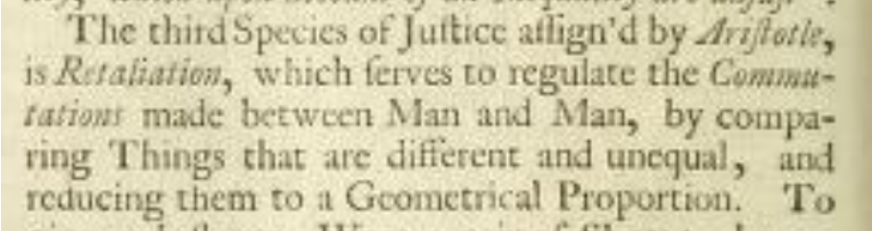
\includegraphics[width=0.79\linewidth]{L4-1.png}
                    \captionof{figure}{Extract from the Latin version}
                \end{center}
            \end{minipage}
            \begin{minipage}{0.5\textwidth}
                \begin{center}
                    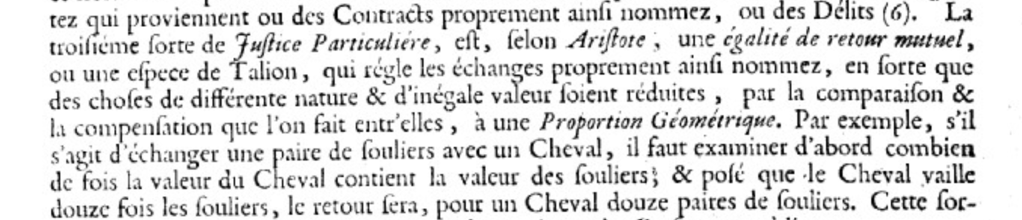
\includegraphics[width=0.99\linewidth]{L4-2.png}
                    \captionof{figure}{Extract from the French version}
                \end{center}
            \end{minipage}

        \subsubsection{The third species of justice}

            The third species of justice is retaliation, by which the exchange of things made by men with one another is governed, while diverse and unequal things made in comparison with each other are finally made equal according to the laws of geometric proportion.

            \begin{example}
                For example, were a pair of shoes to be exchanged for a horse, the question would be, how many times the price of the horse contains the price of the shoes, which supposing to be twelve times, there is compensation if twelve pair of shoes are given for one horse.
            \end{example}

            This specific form of justice, sometimes overlooked, addresses the question of how we exchange unlike goods. Suppose a single horse holds the value of twelve pairs of shoes; the ratio is 1:12. Understanding this ratio allows a fair and geometrically balanced exchange.
    
    \subsection[Of Price cont'd]{Book V, Chapter I\\
                \textit{“Of Price”}}

        Returning to the question of how societies establish measures for such exchanges, Pufendorf further refines the discussion of price in this continuation.

        \subsubsection{Necessity of exchange}

            \begin{quote}
                Since the things subjected to ownership differed in their nature and did not provide the same use for human necessities, and indeed, since frequently it happened either that the same thing (whose parts were not in all respects alike) began to belong to several persons, or that things diverse in nature had to be mutually exchanged, it became necessary that by human agreement some evaluation be imposed on things, according to which those of a disparate nature could be compared and made equal to one another.
            \end{quote}

            He reiterates that as soon as humans possess distinct items—especially when those items serve different purposes—there arises a need for a commonly recognized standard of valuation. This standard must accommodate even goods that are not physically comparable.

        \subsubsection{Coincidence of quantities}

            \begin{quote}
                But since things are compared and made equal to one another by means of a quantitative principle, that is, since equality is a coincidence of quantities, we must now examine the quantity of things and actions insofar as they are useful in human life, as well as this quantity’s foundations and common measure.
            \end{quote}

            It is not just physical attributes that must be compared (size, volume, weight). Rather, humans recognize a deeper notion of equivalence, which Pufendorf calls moral quantity, allowing them to assign a relative worth to otherwise incomparable objects or services.

        \subsubsection{Some quantity beyond the physical and mathematical}

            \begin{quote}
                We find, then, that things are said to be equal to one another in ordinary life not only because they coincide according to the three dimensions, but also in a certain other respect. Thus, honors, labors, and wages are said to be equal or unequal to one another on account of considerations other than the coincidence of their dimensions. So there must be some quantity beyond the physical and mathematical, which philosophers seem thus far to have been exclusively concerned about.
            \end{quote}

            Pufendorf notes that classical philosophy mostly analyzed tangible, measurable features of objects. Yet in commercial societies, the perceived value—shaped by demand, utility, and cultural factors—often proves more decisive than physical dimensions alone.

        \subsubsection{Moral quantities}

            \begin{quote}
                This will be more clear if we attend to the fact that the formal principle of quantity in general consists not in a substance’s extension but, so to speak, its susceptibility to evaluation. In other words, the prime reason things are said to be quantified is that they can be evaluated and, consequently, compared with one another as to their equality or inequality. But since things can be evaluated not only according to their physical substance but also a certain moral consideration, it follows that there is a moral quantity in addition to the physical, according to which they are of course morally evaluated.
            \end{quote}

            This “moral quantity” is an evaluative measure focusing on how useful or desirable a good or service is to potential buyers or the wider community. Hence, price arises from how a society judges an item’s worth, not merely from the item’s physical composition.

    \subsection{Physical quantities for things of the same nature}

        Physical quantity itself does enter into the evaluation of things of the same nature and goodness (for example, other things being equal, a large diamond is worth more than a small one); yet it is not always considered in the evaluation of things differing in kind or goodness. Thus, a bigger dog is not always worth more than a smaller one, nor a large mass of lead more valuable than a smaller mass of gold.

        \subsubsection{Price}

            \begin{definition}[Price]
                This quantity, namely the moral quantity or value according to which things and actions entering into commerce are usually compared with one another, is called price.
            \end{definition}

        \subsubsection{Vulgar and eminent price}

            Price can be divided into vulgar price and eminent price. The former is found in things, and in actions or labours, that enter into commerce, insofar as they afford men some use or pleasure. The latter is found in money and whatever serves in its stead, insofar as it is understood to contain virtually the prices of all things and labours, and to furnish a common measure thereof.

        \subsubsection{Useful things without price}

            It must be observed that some things highly useful to human life are understood to have no price imposed on them. This is either because they are and ought to be exempt from dominion, because they are excluded from human commerce, or finally, when they do enter into commerce, they are never considered otherwise than as an appendage of something else.

        \subsubsection{Price increased by rarity}

            The main factor in a price increase is rarity, whose intentional procurement is considered by some to be among the secrets of the trade... Also, men in general consider hardly anything a good unless it provides its possessor with something more excellent and rare than what others possess.
            
            But this evaluation of genuine goods according to their rarity or the number of people who possess them is in fact due to the wickedness and meanness of the human character. For a good in my possession is surely not made worse by the fact that others have it too, or more excellent if they lack it.

        \subsubsection{But rarity is the exception}

            Hence, their ambition for luxury has imposed enormous prices on many things that human life could very easily have done without. (Some think this was done so that great and enormous riches could have a use.)... But things that are used on a daily basis and that mainly concern food, clothing, and weapons experience their greatest rise in price when they become as rare as they are necessary. This commonly happens during food shortages and sieges, or on long sea voyages, when hunger and thirst demand to be satisfied and life to be preserved at any price.

            \begin{remark}[Usual factors determining the vulgar price]
            
                \begin{itemize}
                    \item the subtlety and elegance of the art which they exhibit
                    \item the fame of the artisan
                    \item the difficulty of the work, the abundance and rarity of artisans or labourers, and similar things
                    \item the price of labours and actions is raised by their difficulty, skill, usefulness, and necessity; and by their agents* rarity, their pre-eminence or stature, their freedom to interrupt the action, and other such things
                    \item the most important factor, however, in the evaluation of a work is the state of the art
                \end{itemize}
            \end{remark}

    \subsection*{Final Considerations}

        In these sections of \textit{De Iure Naturae et Gentium}, Pufendorf demonstrates a comprehensive attempt to systematize natural law by combining classical Aristotelian insights with a modern awareness of commerce and social organization. He thus extends beyond Hobbes’s singular focus on the sanctity of covenants to show that justice encompasses several forms, each intended to address distinct aspects of human relationships—whether distributing shared resources, correcting injustices, or balancing disparate exchanges.

        Ultimately, Pufendorf’s conception of sociability lies at the heart of his theory: human beings, though potentially harmful and self-centered, are compelled by both weakness and reason to live cooperatively. For society to function smoothly, structures of justice—distributive, corrective, and reciprocal—must be respected. Likewise, trading relationships hinge upon shared frameworks of value, articulated as price, which organizes economic life and helps maintain a cohesive social order.

        All these discussions lay important groundwork for subsequent Enlightenment thinkers, shaping modern theories of rights, commerce, and governance. By intricately weaving together moral philosophy, legal theory, and proto-economic analysis, Pufendorf remains a seminal figure in the history of natural law scholarship.